\chapter{Detalii formatare \LaTeX}
\label{chap:main}

\myLettrine{M}{aterialul} curent folosește ca template clasa \textquote{scrrprt} la care s-au adăugat pachete și comenzi uzuale. 

\shadowbox{
\begin{minipage}{.95\textwidth}
Datorită folosirii pachetului \emph{fontspec} ce acceptă în mod nativ diacritice, fișierul sursă latex se poate compila doar cu \textbf{xelatex}, nu și cu \textbf{pdflatex}.
\end{minipage}
}

Pentru a păstra o structură cât mai compactă fișierele sursă s-au împărțit în următoarele categorii\footnote{Nu este obligatoriu să se păstreze aceeași structură dar este recomandat, pentru a păstra o formatare compactă.}:
\begin{description}[style=nextline]
\item[thesis.tex] reprezintă fișierul \textquote{main} în care toate celelalte fișiere sunt apelate
\item[standard.sty] conține pachetele și comenzile folosite uzual
\item[bib.bib] conține câteva referințe în format \emph{bibtex}; referințe adiționale pot fi adăugate după necesități \url{https://texblog.org/2014/04/22/using-google-scholar-to-download-bibtex-citations/}
\item[upb-authoryear.bbx, upb-authoryear.cbx si romanian.lbx] definesc stilul bibliografic asociat intrărilor din lista bibliografică
\item[gls.tex] conține termeni de glosar ce pot fi adăugați la o \textquote{Listă de termeni} dacă se consideră necesar
\end{description}
Comentarii și scurte explicații (în engleză) referitor la rolul pachetelor și comenzilor se regasesc în aceste fișiere sursă.

Adițional, următoarea structură de dosare a fost folosită:
\begin{description}[style=nextline]
\item[cls] pentru stocarea fișierelor-sursă auxiliare (pentru introducerea de pachete/referințe bibliografice, etc.)
\item[pics] pentru stocarea imaginilor ce vor fi adaugate în manuscris
\item[chapters] pentru stocarea fișierelor \textquote{capitol} (pentru ușurința în lucru, am presupus că textul fiecărui capitol va fi pus într-un fișier sursă de sine-stătător)
\item[code] pentru stocarea fișierelor \textquote{sursă} ce vor fi apoi adăugate în manuscris
\end{description}

\begin{rem}
\label{rem:at}
În cazul în care se dorește modificarea structurii mai sus-menționate, o atenție sporită trebuie acordată referințelor făcute în cadrul fișierelor. \eor
\end{rem}

Fișierele au fost compilate folosind distribuția Miktex 2.9 (\url{http://miktex.org/2.9/setup}), cu ajutorul editorului de text TexnicCenter (\url{http://www.texniccenter.org/}). Detalii generale despre \LaTeX se pot găsi de exemplu în \url{http://tobi.oetiker.ch/lshort/lshort.pdf}. În cele ce urmează sunt prezentate câteva situații tipice.


\section{Exemple comenzi de tip float}
În această secțiune  vor fi exemplificate câteva construcții de tip \textquote{float}. În general, fiecărui float i se poate asocia un element de tip \emph{legendă} pentru a putea da o explicație detaliată și un element de tip \emph{etichetă}, ce va permite referirea la acest float în cadrul manuscrisului cât și enumerarea sa în cadrul listei asociate (de exemplu in \emph{lista de figuri} vor apare toate figurile definite în manuscris).

\subsection{Tabele}
Informații suplimentare despre tabele pot fi gâsite de exemplu în \url{http://en.wikibooks.org/wiki/LaTeX/Tables}.
Câteva exemple simple sunt ilustrate în continuare.

\begin{table}[ht!]
\begin{tabular}{llll}
\hline
Fault & Fault & Symbol & Type\\ 
No. & & & \\
\hline
1 & Sensor Fault & $\Delta\beta_{1,m1}$ & Fixed Value\\
2 & Sensor Fault & $\Delta\beta_{2,m2}$ & Gain Factor\\
3 & Sensor Fault & $\Delta\beta_{3,m1}$ & Fixed Value\\
4 & Sensor Fault & $\Delta\omega_{r,m1}$ & Fixed Value\\
5 & Sensor Fault & $\Delta\omega_{r,m2}$, $\Delta\omega_{g,m2}$ & Gain Factor\\ 
\hline
\end{tabular}
\centering
\caption{Faults affecting the wind turbine model}%Considered Faults}
\label{tab:faults}
\end{table}

\begin{table}[ht!]
\begin{center}
\begin{tabular}{|c|c|c|c|c|c|c|c|}
\hline
no. of hyperplanes&5&10&15&20&25&50&100\\ \hline
classical&9.91&64.06&91.74&511.47&306.04&$\cdots$&$\cdots$\\ \hline
enhanced&1.14&0.81&0.59&4.84&4.18&3.66&2.94\\ \hline
\end{tabular}
\end{center}
\caption{Numerical values for the solving of an MI optimization problem under classical and anhanced methods.}
\label{tab:run}
\end{table}

Atât \tabref{tab:faults} cât și \tabref{tab:run} vor aparea în lista de tabele și vor putea fi referite în text cu ajutorul etichetei asociate fiecăruia.

\subsection{Figuri}
În mod similar se pot afișa diverse imagini (se recomandă fie imagini în format raster de rezoluție suficientă, fie imagini in format vectorial -- eps, pdf, tikz). Detalii suplimentare se pot găsi de exemplu în \url{http://en.wikibooks.org/wiki/LaTeX/Floats,_Figures_and_Captions}.

\begin{figure}[!ht]
\begin{center}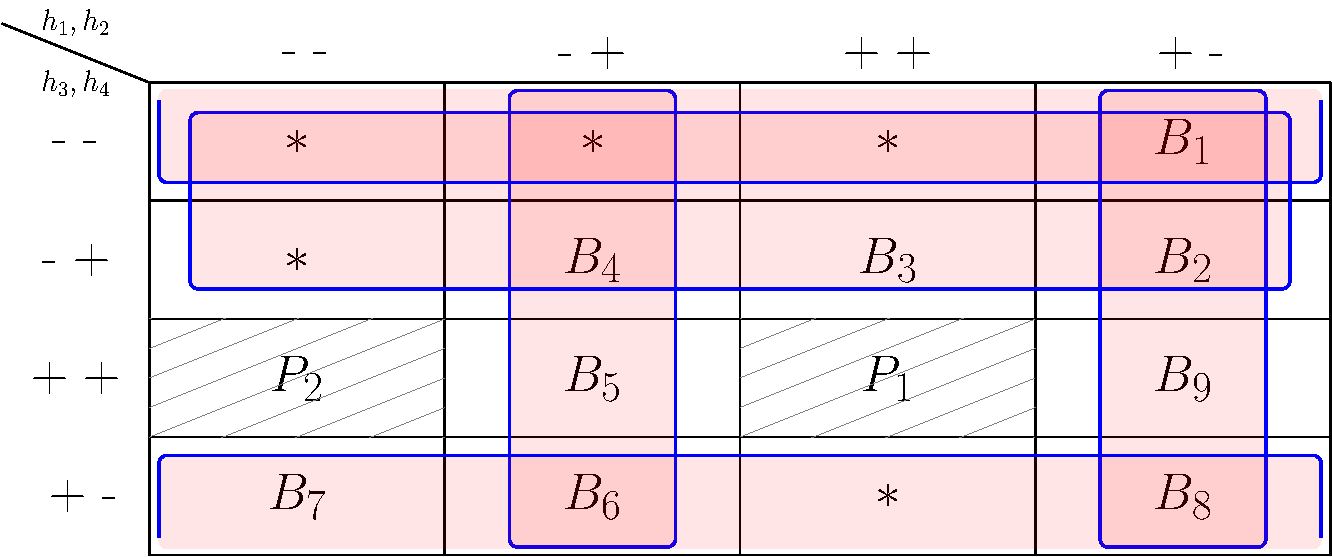
\includegraphics[width=\singlefigure]{\pics/binary/KarnaughDiagramForHyperplaneArrangement}\end{center}
	\caption{Karnaugh diagram for obaining the reduced cell representation}
	\label{fig:karnaugh}
\end{figure}

În \figref{fig:karnaugh} se ilustrează un exemplu simplu (o singură figură) iar în \figref{fig:int} se face uz de pachetul \textquote{subfig} ce permite o structură de tip tabel cu mai multe sub-figuri (fiecare dintre acestea poate fi referită în mod independent -- de exemplu, \figref{fig:int}\subref{fig:intc}).

\begin{figure}[!ht]
\begin{center}
  \subfloat[cut for each tuple]{\label{fig:inta}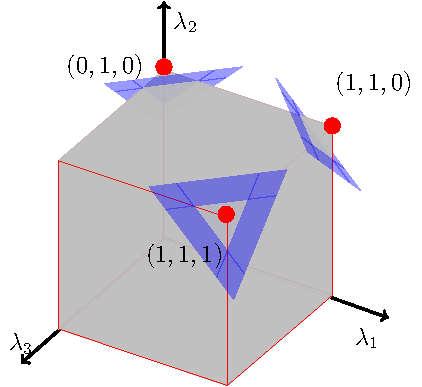
\includegraphics[width=\triplefigure]{\pics/binary/cutForEveryTuple}}
	\subfloat[cut for each complete face]{\label{fig:intb}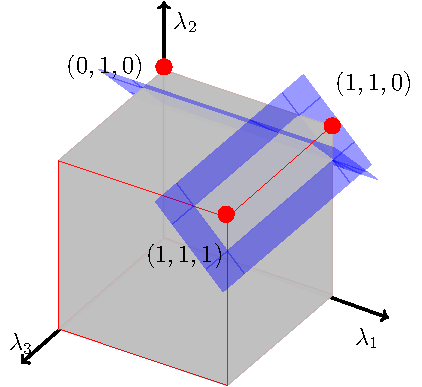
\includegraphics[width=\triplefigure]{\pics/binary/cutForEveryEdge}}
	\subfloat[only one cut]{\label{fig:intc}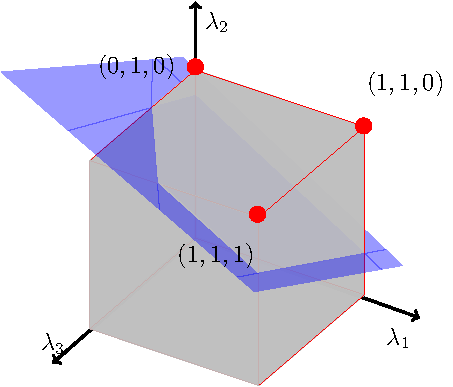
\includegraphics[width=\triplefigure]{\pics/binary/cutForAllTuples}}
	\caption{Exemplification of separating hyperplanes techniques}
	\label{fig:int}
\end{center}
\end{figure}


\begin{rem}
Dimensiunea unei figuri este determinată de argumentul opțional `width'. S-a preferat folosirea de macro-uri (\verb+\singlefigure+ și \verb+\triplefigure+) și nu valori \textquote{hard-coded} datorita flexibilității lor. Shimbând în preambul (în \emph{standard.sty}) valoarea unui astfel de macro se vor schimba automat dimensiunile figurilor ce îl folosesc, fără a mai fi nevoie să se modifice fiecare în parte. \eor
\end{rem}

\subsection{Algoritmi}

În exemplul de mai jos, \algref{alg:run} folosește pachetul \textquote{algorithm2e} pentru redactarea unui algoritm. Prin modificarea opțiunilor din preambulul documentului (în \emph{standard.sty}) este posibilă modificarea structurii/introducerea de noi cuvinte cheie/etc.

\begin{algorithm2e}
\caption{Fault tolerant scheme}
\label{alg:run}
\KwIn{$\mathcal{I}=\mathcal{I}_H(0)\cup \mathcal{I}_F(0);\quad\mathcal{I}_H(0)\neq \emptyset$}
$k \leftarrow$ the current sampling time\;
\ForEach{sensor $i\in \mathcal{I}_F(k-1)$}{
	\If{$r_i(k-1)\in R_i^F$ and $r_i(k) \in R_i^H$}{compute a timer $\bar \theta_i$ \;}
	}
\end{algorithm2e}

\section{Lista bibliografică}

Lista bibliografică este extrasă dintr-un fișier \textquote{*.bib} în care sunt stocate articole/cărți/conferințe în format bibtex (detalii suplimentare pot fi gasite la \url{http://en.wikibooks.org/wiki/LaTeX/Bibliography_Management}). Un exemplu al unei astfel de intrări este:


\begin{verbatim}
@article{gilbert1991linear,
 title={{Linear systems with state and control constraints: the theory and application of maximal output admissible sets}},
 author={Gilbert, EG and Tan, KT},
 journal={IEEE Transactions on Automatic Control},
 volume={36},
 number={9},
 pages={1008--1020},
 year={1991}
}
\end{verbatim}

Pentru citarea în text și listarea intrărilor citate în lista bibliografică s-a folosit pachetul \textquote{biblatex}. În cadrul acestui pachet, cele mai uzuale comenzi de citare sunt următoarele:
\begin{description}[style=nextline]
\item[citare simplă] \verb+\cite{...}+: \cite{bitsoris2006invariance}
\item[citare pusă între paranteze] \verb+\parencite{...}+: \parencite{gilbert1991linear}
\item[citare cu anul pus între paranteze] \verb+\textcite{...}+: \textcite{loechner1999polylib}
\item[citare cu intrări multiple] \verb+\cite{..., ..., ...}+: \cite{bellingham2002receding,garey1979computers,vitus_tunnel-milp:_2008,camponogara2002distributed}
\end{description}

În mod automat, intrările citate în text (și doar ele) vor fi puse în lista de referințe de la sfârșitul manuscrisului.


\section{Localizare: română versus engleză}

În fișierul principal (\emph{thesis.tex}), prin selectarea opțiunii \emph{language=english}, \emph{language=romanian} se poate alterna, respectiv, între formatarea în engleză și cea în română a textului. Câteva exemple sunt:
\begin{itemize}
\item numele cuprins-ului va alterna între \textquote{contents/cuprins}
\item în interiorul listei bibliografice caracterele de legatură se vor adapta (de exemplu, `and' devine `și')
\item \textquote{ghilimelele} se vor adapta la limba folosită (daca pentru a cita un fragment de text folosiți comenzile \verb+\textquote+ sau \verb+\blockquote+)
\item blocurile matematice își vor schimba eticheta, de exemplu `Theorem' devine `Teorema' 
\item referința la un element, de exemplu `Figure 2.3' devine `Figura 2.3'
\end{itemize}

Pentru diacritice (\u a,\^ a,\^ i, \c s, \c t etc.) se poate recurge fie la o codare explicită (\verb+\u a+, \verb+\^ a+, \verb+\^ i+, \verb+\c s+, \verb+\c t+) așa cum e detaliat în \url{http://en.wikibooks.org/wiki/LaTeX/Special_Characters} fie la scrierea lor direct de la o tastatura setată în limba romana într-un editor de text ce suportă utf8.


\section{Diverse}

\begin{description}[style=nextline]
\item[blocuri matematice] pentru blocurile tipic întălnite în matematică (Teoremă, Propoziție, Definiție, Remarcă, etc.) există definiții în preambul ce permit notarea/etichetarea și apelarea lor în mod automat. Spre exemplu, un bloc de tip teoremă se scrie astfel:

\begin{thm}
\label{thm:test}
Conținut teoremă ... urmat de simbolul de terminare a textului. \eot
\end{thm}
\begin{proof}
Demonstrație a afirmațiilor făcute în teoremă.
\end{proof}
Teorema poate fi apoi referită în text prin intermediul etichetei sale: \thmref{thm:test}.
\item[referințe în text]
Cu ajutorul etichetelor asociate blocurilor definite în latex, este posibilă referirea în mod automat a acestor elemente oriunde în manuscris. Prin adaugarea pachetului \emph{hyperref} aceste referințe devin link-uri ce fac legătura cu elementul față de care sunt asociate.
 
Exemple de referințe pot fi ecuații (\eqref{eq:test}), elemente de structură (\chapref{chap:intro}), blocuri matematice (\remref{rem:at}) sau figuri/tabele/algoritmi. Pentru multe dintre acestea,  în fișierele sursă s-au definit macro-uri. Deși nu este obligatoriu, recomandăm uzul acestora datorita flexibilității lor. De exemplu, folosind \verb+\figref{eticheta}+ putem să ne adaptam în mod automat la schimbarea limbajului de lucru (în preambul, acest macro va schimba, în funcție de opțiunea aleasă, între `Figure' și `Figura').

\item[termeni de glosar, acronime]
În fișierul \emph{./cls/gls.tex} introduceți termeni de glosar. Aceștia pot fi apoi folosiți prin apelarea comenzii \verb+\gls{numeTermen}+. Spre exemplu \gls{computer} este un termen de glosar iar \gls{fpsLabel} și \gls{lvm} sunt acronime (atunci când sunt apelate prima oară apar în forma desfășurată, la următorele apelări apar doar cu abreviere: \gls{fpsLabel} și \gls{lvm}). Acești termeni vor fi enumerați într-o listă de termeni de glosar / acronime la începutul lucrării.

Detalii suplimentare pot fi găsite la pagina \url{https://en.wikibooks.org/wiki/LaTeX/Glossary} sau în documentul \url{http://ctan.math.utah.edu/tex-archive/macros/latex/contrib/glossaries/glossariesbegin.pdf}.

\item[fragmente de cod] 
Cu ajutorul pachetului \emph{listings} este posibilă afișarea fragmentelor de cod relevante pentru document prin referirea către un fișier sursă existent (ceea ce înseamnă ca orice modificare a acestuia se va reflecta automat în textul afișat).

Spre exemplu:  în \lstref{lst:s1} este afișat un întreg fișier sursă iar în \lstref{lst:s2} sunt afișate liniile 5-15 din alt fișier sursă folosind comenzile:

%\begin{Verbatim}[samepage=true]
%\lstinputlisting[caption={Cod Matlab -- fișier complet},label={lst:s1}]{\code/s1.m}
%\lstinputlisting[caption={Cod Matlab -- fragment de fișier},label={lst:s2},firstline=5,lastline=15]%{\code/s2.m}
%\end{Verbatim}

\end{description}


\section*{Disclaimer}

Acest ghid de redactare este încă într-o versiune preliminară. Ca atare, diverse erori/bug-uri sunt posibile. Dacă întălniți astfel de situații aduceți-mi-le la cunoștiință la adresa \href{mailto:florin.stoican@acse.pub.ro}{florin.stoican@acse.pub.ro} sau pe forum-ul din cursul asociat lucrării de licență de pe Moodle.